\section{Introduction}\label{introduction}

\begin{frame}{Path finding as decision problems}

Given two nodes \clr{red}{$a$} and \clr{blue}{$b$} in a graph $G$, is
there a path from \clr{red}{$a$} to \clr{blue}{$b$}?

\begin{description}
\item[$PATH$]
for directed graphs
\item[$UPATH$]
for undirected graphs
\end{description}

\begin{center}
\begin{tikzpicture}[->,line join=bevel, thick]
  \tikzstyle{vertex}=[circle,fill=black!25,minimum size=12pt,inner sep=2pt]
  \node[vertex, fill=blue!25] (a) at (0,1)  {a};
  \node[vertex, fill=red!25] (b) at (4,0)  {b};
  \node[vertex] (1) at (2,0)  {};
  \node[vertex] (2) at (1,2)  {};
  \node[vertex] (3) at (3,2)  {};
  \node[vertex] (4) at (5,2)  {};
  \node[vertex, fill=green!25] (c) at (4,2)  {c};
  \path (a) edge [bend right]  (1)
        (1) edge [bend left]  (2)
        (3) edge [loop]  (3)
        (3) edge [bend left]  (1)
        (1) edge (b)
        (2) edge [bend left]  (3)
        (4) edge (c);
  \path (a) edge [bend right, visible on=<2->, orange]  (1)
        (1) edge [bend left, visible on=<2->, orange]  (2)
        (3) edge [loop]  (3)
        (3) edge [bend left, visible on=<2->, orange]  (1)
        (1) edge [visible on=<2->, orange] (b)
        (2) edge [bend left, visible on=<2->, orange]  (3);
\end{tikzpicture}
\end{center}

\begin{block}
\only<2>{$\Rightarrow (a, b, G) \in PATH$, but $(a, c, G) \not \in PATH$}
\end{block}

\end{frame}

\begin{frame}{$UPATH$ vs. $PATH$}

\begin{itemize}
\item
  Seem similar, but can be used to charaterize the space complexity
  classes $L$ and $NL$
\item
  Using \emph{randomization} we can solve $UPATH$ without
  non-determinism only using logarithmic bounded space
\item
  This algorithm is called \emph{RandomWalk}
\item
  $PATH$ however is $NL$-complete
\item
  Note: $PATH$ \emph{could} be just as easy as $UPATH$ if $L = NL$
\end{itemize}

\end{frame}

\begin{frame}{Random Walk}

\begin{center}
\begin{tikzpicture}[line join=bevel, thick, every loop/.style={}]
  \tikzstyle{vertex}=[circle,fill=black!25,minimum size=12pt,inner sep=2pt]
  \tikzstyle{vertex_marked}=[vertex,fill=orange!25]
  \node[vertex, fill=blue!25] (a) at (0,1)  {a};
  \node[vertex, fill=red!25] (b) at (4,0)  {b};
  \node[vertex] (1) at (2,0)  {$v_1$};
  \node[vertex] (2) at (1,2)  {$v_2$};
  \node[vertex] (3) at (3,2)  {$v_3$};
  \node[vertex] (4) at (5,2)  {$v_4$};
  \node[vertex, fill=green!25] (c) at (4,2)  {c};
  \path (a) edge [bend right]  (1)
        (1) edge [bend left]  (2)
        (3) edge [loop]  (3)
        (3) edge [bend left]  (1)
        (1) edge (b)
        (2) edge [bend left]  (3)
        (4) edge (c);


  \path (a) edge [->, bend right, orange, visible on=<2-2>]  (1)

        (1) edge [->, bend left, orange, visible on=<4-4>]  (2)
        (1) edge [->, bend right, orange, visible on=<4-4>]  (3)
        (1) edge [->, orange, visible on=<4-4>]  (b)

        (3) edge [->, loop, orange, visible on=<6-7>]  (3)
        (3) edge [->, bend left, orange, visible on=<6-7>]  (1)
        (3) edge [->, bend right, orange, visible on=<6-7>]  (2)

        (1) edge [->, bend left, orange, visible on=<9-9>]  (2)
        (1) edge [->, bend right, orange, visible on=<9-9>]  (3)
        (1) edge [->, orange, visible on=<9-9>]  (b);

  \node[visible on=<1->, vertex, fill=blue!25] (a) at (0,-2)  {a};
  \node[visible on=<3->, vertex]               (1) at (1,-2)  {$v_1$};
  \node[visible on=<5->, vertex]               (3) at (2,-2)  {$v_3$};
  \node[visible on=<7->, vertex]               (3) at (3,-2)  {$v_3$};
  \node[visible on=<8->, vertex]               (1) at (4,-2)  {$v_1$};
  \node[visible on=<10->, vertex, fill=red!25]  (b) at (5,-2)  {b};

  \node[vertex_marked, visible on=<1-2>] (a_marked) at (0,1)  {a};
  \node[vertex_marked, visible on=<3-4>] (1_marked) at (2,0)  {$v_1$};
  \node[vertex_marked, visible on=<5-7>] (3_marked) at (3,2)  {$v_3$};
  \node[vertex_marked, visible on=<8-9>] (1_marked) at (2,0)  {$v_1$};
  \node[vertex_marked, visible on=<10-10>] (b_marked) at (4,0)  {b};

\end{tikzpicture}
\end{center}

\end{frame}

\begin{frame}{Universal Traversal Sequence}

\begin{itemize}
\item
  Route description that works on \emph{all} (connected) d-regular
  Graphs of a certain size $n$
\item
  Example for $d = 3$ and $n = 4$:
\end{itemize}

\begin{center}
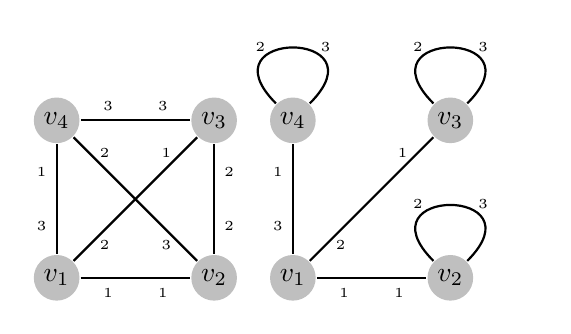
\begin{tikzpicture}[line join=bevel, thick, every loop/.style={}]
  \tikzstyle{vertex}=[circle,fill=black!25,minimum size=12pt,inner sep=2pt]
  \tikzstyle{edge_label}=[font=\tiny]
  \node[vertex] (1) at (0,0)  {$v_1$};
  \node[vertex] (2) at (2,0)  {$v_2$};
  \node[vertex] (3) at (2,2)  {$v_3$};
  \node[vertex] (4) at (0,2)  {$v_4$};
  \node[vertex] (1b) at (3,0)  {$v_1$};
  \node[vertex] (2b) at (5,0)  {$v_2$};
  \node[vertex] (3b) at (5,2)  {$v_3$};
  \node[vertex] (4b) at (3,2)  {$v_4$};
  \path (1) edge node [edge_label, near start, below] {1} node [edge_label, near end, below] {1} (2)
        (1) edge node [edge_label, near start, below] {2} node [edge_label, near end, above] {1} (3)
        (1) edge node [edge_label, near start, left] {3} node [edge_label, near end, left] {1} (4)
        (2) edge node [edge_label, near start, right] {2} node [edge_label, near end, right] {2} (3)
        (2) edge node [edge_label, near start, below] {3} node [edge_label, near end, above] {2} (4)
        (3) edge node [edge_label, near start, above] {3} node [edge_label, near end, above] {3} (4);

  \path (1b) edge node [edge_label, near start, below] {1} node [edge_label, near end, below] {1} (2b)
        (1b) edge node [edge_label, near start, below] {2} node [edge_label, near end, above] {1} (3b)
        (1b) edge node [edge_label, near start, left] {3} node [edge_label, near end, left] {1} (4b)
        (2b) edge [loop] node [edge_label, near start, above] {3} node [edge_label, near end, above] {2} (2b)
        (3b) edge [loop] node [edge_label, near start, above] {3} node [edge_label, near end, above] {2} (3b)
        (4b) edge [loop] node [edge_label, near start, above] {3} node [edge_label, near end, above] {2} (4b);

\end{tikzpicture}
\end{center}

Universal Traversal Sequence: $(1, 2, 3, 2, 1, 1, 2, 1, 3, 1, 2)$

\end{frame}

\section{Space-Complexity}\label{space-complexity}

\begin{frame}{Space-Complexity classes L and NL}

\begin{itemize}
\item
  Input already occupies $n$ cells.
\item
  Seperate space usage of input/output from computation
\item
  We need a different turing machine model, with 3 tapes:

  \begin{itemize}
  \itemsep1pt\parskip0pt\parsep0pt
  \item
    1 read-only input tape
  \item
    1 read/write work tape
  \item
    1 write-only output tape
  \end{itemize}
\item
  Head of input tape \emph{must} remain on the input (+ a
  \emph{constant} offset)
\item
  $L = DSPACE(\log n)$
\item
  $NL = NSPACE(\log n)$
\item
  As with $P = NP$, $L = NL$ is also still unknown
\end{itemize}

\end{frame}

\begin{frame}{Examples for problems that can be solved in $L$}

\begin{description}
  \item[\textit{Counting all occurences of a symbol in the input}] \hfill \\
    $\log n$ bits for the current count
  \item[\textit{Maximum distance between symbols}] \hfill \\
    counter for current distance and current maximum
  \item[\textit{Write down all positions of a certain symbol}] \hfill \\
    counter for current position. The output is in $O(n \cdot \log n)$
\end{description}

\end{frame}

\begin{frame}{$NL \subseteq P$}

\begin{theorem}
The running time of every log-space bounded turing machine is bounded by a polynominal.
\end{theorem}

\begin{block}
\visible<1-1>{
\begin{itemize}
\item Configuration: Position of input and working heads, current state of working tape, current state
\item The possible positions of the input head are bounded by $n +c_1$
\item The possible positions of the working head are bounded by $\log n + c_2$
\item The possible states of the working tape are bounded by $\Gamma^{\log n + c} \in O(n^k)$
\item The number of possible states (or sets of states) in constant with regard to the input size
\item $(n + c_1) \cdot (\log n + c_2) \cdot n^k \in O(n^{k+2})$
\end{itemize}
}
\onslide<2->{
Foo
}
\end{block}

\end{frame}

\begin{frame}{PATH is NL-complete}

\begin{itemize}
\itemsep1pt\parskip0pt\parsep0pt
\item
  Informal definition of NL-completeness:

  \begin{itemize}
  \itemsep1pt\parskip0pt\parsep0pt
  \item
    Transform instance of decision problem A to instance for B and use B
    to solve it
  \item
    Restrict power of transformation function
  \end{itemize}
\item
  More precisely cover the transformation: TM -\textgreater{}
  configuration graph

  \begin{itemize}
  \itemsep1pt\parskip0pt\parsep0pt
  \item
    only log-bounded space needed to encode current configuration
  \item
    look at possible next configurations and write to output tape
  \end{itemize}
\item
  Applying PATH to that should be trivial
\end{itemize}

\end{frame}

\section{RL and RandomWalk}\label{rl-and-randomwalk}

\begin{itemize}
\item
  Use RandomWalk to construct randomized decider for $UPATH$
\item
  Show that it can not work for $PATH$
\end{itemize}

\begin{frame}{Proofing a bound on the number of steps}

\begin{itemize}
\item
  Short example of Markov-Chain
\item
  Relation to RandomWalk: Important connected graph
\item
  RandomWalk can be modeled as Markov-Chain (Markov Property)
\item
  Derive expected length of a random walk starting at any node $a$ to
  reach any other node $b$: We proof an upper bound: Expected number of
  steps to visit all nodes in G.
\item
  Overview:
\item
  First compute $P_v$ and thus $E(v, v)$
\item
  Compute upper bound for $E(u, v)$
\item
  Compute upper bound for $E(a, G)$
\item
  Apply Markov-Inequality to compute probaboility that we need more than
  8\emph{e}n steps.
\end{itemize}

\end{frame}

\section{Universal Traversal
Sequences}\label{universal-traversal-sequences}

\begin{frame}{d-regular graphs}

\begin{itemize}
\itemsep1pt\parskip0pt\parsep0pt
\item
  Definition
\item
  Number of d-regular graphs of size n
\item
  Traversal sequences and random walks
\end{itemize}

\end{frame}

\begin{frame}{Probability amplification}

\begin{itemize}
\itemsep1pt\parskip0pt\parsep0pt
\item
  Conduct $m$ random walks, probability of not finding a path is
  $2^{-m}$, but size only $8en \cdot m$
\item
  Make $m$ big enough that the probability of a given traversal
  sequences to work for all graphs is bigger than 0:

  \begin{itemize}
  \itemsep1pt\parskip0pt\parsep0pt
  \item
    Again markov inequality: $E(F) = g_{n, d} \cdot 2^{-m} < 1$, thus:
    $1 - Pr[F < 1] = Pr[F \geq 1] \leq E(F) / 1$ \textless{} 1 which
    results in $0 < Pr[F < 1]$
  \end{itemize}
\end{itemize}

\end{frame}
